\chapter{Building a statewide model for state needs}\label{sec:building-models}

There is broad consensus on best practices for trip-based travel models in urban areas, and an abundance of literature to inform the development. Activity-based person travel models likewise tend to have similar components, with choices arranged in comparable order, despite their continuing evolution. Developers and users of such models can point to the best features of each, and a considerable of research is underway to improve them. It is more difficult to portray a typical statewide travel model. They address a wider range of requirements, cover much larger areas, and focus on markets that are not as well understood as those in urban areas.

This chapter attempts to overcome that by describing how such models are built, and the resources required to do so. It begins with a discussion of the foundations necessary to undertake statewide modeling, to include the geographic extent of such models, and how the economy, society, and transportation networks are represented. Trip and activity-based person and freight travel models are described in the following sections. They are followed by an examination of issues relating to integrating urban and statewide models, model validation, and the computational burdens associated with statewide modeling.

It is important to note that this chapter does not attempt to describe best practices in statewide modeling. What is best for any given agency is contextual, defined by their intended uses of the model. The best model is arguably one that addresses their needs promptly, with the least amount of investment, and which their staff can creatively and competently apply. Those dimensions are not addressed in this chapter. Rather, an attempt is made to define the state of the art and likely costs and benefit of pursuing it.

The costs described are based upon a review of the data collected for this report, costs described in the literature and model documentation, and experience of the authors. The costs shown for data are only for their acquisition. The cost of transforming them into models is stated in terms of typical additional cost for consultants to do so. Ideally, this work would be done by agency staff, to instill the skills and institutional knowledge required to maximize the investment in data and models. The cost savings associated with doing so are not addressed, for they likely vary widely.

The discussion of options presented in this chapter is limited to operational models, or those close to becoming so. There are many promising lines of ongoing research that might change how we build and use statewide models, as well as prototypes built by researchers and practitioners alike. However, these are typically not mature enough or proven in practice to include here. Moreover, it is difficult to guess at what data requirements they might have or their full cost of implementation.

\section{The modeling environment}

We can consider the modeling environment apart from the models applied within it. The former includes how the demographic and land use markets in the modeled area are represented, as well as the multimodal transportation network and service providers. The state and regional economy are increasingly being represented in statewide models are well. Most often decisions about the desired levels of spatial, temporal, and behavioral resolution are made on this basis. That is, the agency's needs frame the required level of detail in the model, not the other way around. However, those parameters differ by model component. The economy, land use, and travel choices all evolve at different rates, and are best represented at different geographic and time scales. This is especially true for long-distance models, where it is usually sufficient to know the state or megaregion of distal trip ends.

Early statewide models tackled the issue of conflicting resolutions by modeling the entire system at the highest level of resolution required for any of its components. Such an approach makes sense when only modeling travel choices. However, attempting to model the regional economy at the traffic analysis zone quickly proves intractable, for the rich time series of macroeconomic data extends from the national level down to counties, but not below it. It is possible to divide the data into successively smaller units, but a more flexible approach is to develop modeling systems that operate at multiple levels. There is a long tradition of doing so for freight models that can be extended into statewide models. \cite{xu03} describes a multi-level national model, in which financial, supply chain, and transport markets are represented at different levels of resolution, as shown in Figure \ref{fig:multi-scale-modeling}. Microsimulation approaches are more amenable to operating at several levels than aggregate models, making these easier to integrate into activity-based models.

\begin{figure}  % 43
\centering
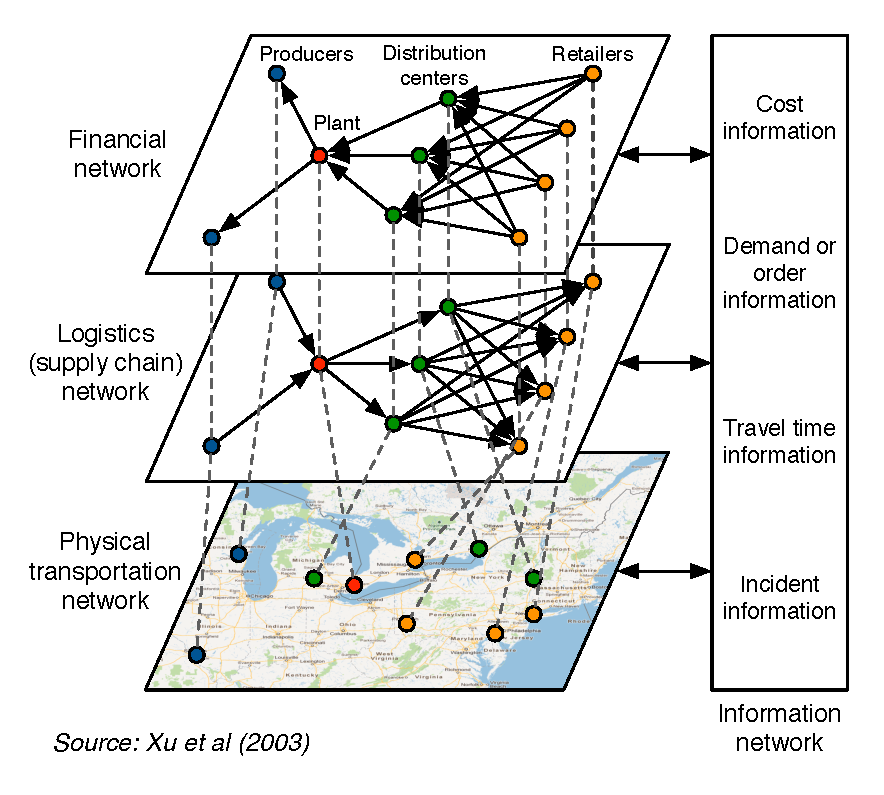
\includegraphics[scale=0.6]{graphics/43-multi-scale-modeling}
\caption{Multi-scale modeling framework}
\label{fig:multi-scale-modeling}
\end{figure}

A model incorporating multiple levels of geography can also use networks scaled to each, although no operational model is known to do so. Rather, most analysts aggregate travel time and distance skims from the statewide model to levels represented at coarser levels of geography, providing them with measures of spatial separation instead of multiple networks. Agents representing households and firms can easily incorporate data from different levels, while reconciling flows between networks of differing resolution remains a very difficult proposition.

\subsection{External markets}

Many decision-makers are interested in knowing from where people and goods move into and out of the state. This is especially true in so-called ``bridge states,'' who feel the impact of large numbers of through trips that do not contribute to its economy. This is also true for freight shipments, which are increasingly part of global supply chains. Representing these external markets, and the flows coming to and from them, has historically been a challenge for statewide modelers. The amount of work required to explicitly include them, as well as the paucity of data, have limited the options for modelers.

Building an external zone system that covers the rest of North America, and populating it with Census and Commerce data about aggregate activity levels, is straight-forward. Obtaining forecasts for those attributes, on the other hand, has historically been challenging and expensive. However, even more difficult was obtaining robust data on the person and freight flows between them. This changed quickly for freight with the introduction of the FAF (\S\ref{sec:traditional-freight-data}), which has improved continually since then. Using the 146 FAF regions covering North America to represent the rest of the continent makes summarization of these data simple.

Comparable data are not available for long-distance person travel, except for the small amount of NHTS long-distance data coded to the Census region level. This obviates the need to consider their geographic representation in addition to, or in lieu of, the FAF regions. If the national person and freight models described in \S\ref{sec:national-model-integration} were to become operational their data would be available at much finer levels of geography. Including the FAF regions as placeholders for their eventual use will quickly add a national context to existing models.

\subsection{Macroeconomic data and models}

Most states use economic forecasts prepared by third parties, including other state agencies and commercial products. The types of data provided range from employment estimates to gross state product by industry that vary by level of geographic and industry detail, and how far into the future estimates are provided for. Many only include the state being modeled, although several states have calculated the growth rates implicit in the FAF to learn where growth in external markets is likely to occur.

Incorporating economic forecasts into existing statewide models is straight-forward, although they are typically provided at the statewide or metropolitan region level. Using these data to drive future estimates of population and employment, either at the zonal level or in synthetic populations, is relatively straight-forward.

A few states have attempted to include an economic model within their statewide modeling system. This is normally done within the context of an integrated economic-land use-transport modeling system, such as those in Ohio and Oregon. An agency might consider building such a model to create better and more internally consistent demographic forecasts. They might also wish to evaluate how changes in travel costs and accessibility influence economic growth, or the consequences of loss or degradation of portions of the network. However, the costs associated with building such a model, and the multi-year development cycles, often make this a prohibitively expensive undertaking unless dictated by agency or legislative reporting requirements.

\subsection{Multimodal networks}

Building and maintaining networks remain a heavy burden at all levels of travel demand modeling, as discussed in \S\ref{sec:network-representations}. Advances in this realm have been small compared to other aspects of modeling. Most statewide models appeared to only include major arterials and higher functional class roadways within the state, and Interstate and numbered U.S. highways outside of it. The National Highway Planning Network or Oak Ridge Network (used for coding the CFS and assigning FAF flows) are typically adapted for this purpose. Fixed guideway and intercity rail transit lines are usually explicit, although local bus service is not. \cite{circella14} describe a straightforward method of synthesizing such coverage in statewide models that greatly reduces the burden associated with representing local transit service, and seems appropriate for most statewide models.

Additional network detail is often desired, to support project-level and small area analyses with statewide models. Indeed, some states do include all roadways, down to the collector and local road level, in their models. None have documented benefits other than the ability to support detailed analyses, or the additional cost involved. Thus, we can only rely upon anecdotal evidence that suggests that doing so greatly increases the amount of work involved. Whether it is worth the investment is a question that only the agency can answer.

\section{The modeling approaches}

Most statewide models are trip-based formulations, very similar in structure to comparable urban models. They often have simplified or no mode choice models, especially in places where intercity transit has a very small market share. Those that have trip-based person models are also likely to have trip-based freight models as well. Many of these models are created with transferred or synthetic data, as revealed in Table \ref{tab:data-combinations} (page \pageref{tab:data-combinations}). Only three states --- California, Ohio, and Oregon --- have implemented an activity-based person modeling approach, all of which also use tour-based truck models.

\subsection{Trip-based person modeling approaches}

The trip-based modeling paradigm is well established, with well-known requirements for their development and deployment. Several states have built models that meet their needs with no more than such knowledge, transferable parameters from the NCHRP reports listed in \S\ref{sec:traditional-person}, and summaries derived from the ACS PUMS data and NHTS microdata. They almost always lack a mode choice modeling component, but are otherwise a competent implementation of best practices in trip-based models. Thus, it is demonstrably easy to build a first-generation model once the initial, and often costly, investment has been made in developing the modeling backplane.

There are several paths past this initial implementation when remaining within a trip-based modeling paradigm. An exhaustive list is beyond the scope of this discussion, but some of the most commonly pursued paths include:

\begin{itemize}
\item
Some states have conducted statewide travel surveys, fused urban travel surveys within their state (and sometimes adjacent ones), or relied upon urban surveys for those with one dominant metropolitan area, to derive trip characteristics used in the model (e.g., trip production and attractions, trip length frequency and time-of-day distributions). Michigan and Oregon have fielded surveys designed to capture adequate samples in different regions of the state. The existing model can be updated using these data, or extended with new features or greater detail.
\item
Other states need to develop mode choice and network assignment capabilities that facilitate pricing analyses. The auto nest of urban and intercity mode choice models can be extended to include pricing, which requires asserting and calibrating the coefficients associated with the new sub-nest(s), based on experience elsewhere, or conducting or adapting additional RP or SP surveys. An RP/SP survey of the size and scope recently conducted for the California HSR modeling work, described in \S\ref{sec:california-hsr-model}, is necessary for estimating a model specific for the modeled area. The cost of that survey was approximately \$350,000. Thus, depending upon the data available and approach chosen this enhancement likely represents a significant investment.
\item
Replacing a traditional trip distribution model with a logit-based destination choice model often leads to improvements in model validation and explanatory power. Such models are usually estimated using existing travel survey data, which often requires adding occupation to the list of variables generated for synthetic populations or zonal estimates. However, the recent availability of OD matrices based on cellular tracking, with their ability to partition flows by residents versus visitors and trip purpose, is a huge advance that will revolutionize travel modeling. Their cost depends upon the geographic scale and duration of data provided. The expected cost of these data, ranging from \$250,000 to \$2M, should be factored into the cost of all statewide models in the future.
\item
Visitor models can be built in several ways. Two broad approaches for doing so have emerged. One uses the same cellular tracking data described above to create visitor flow matrices, to which growth factors can be applied when forecasting. The alternative is to build a synthetic model, based upon the slim survey data available and counts of travelers by mode. \cite{moeckel11} describe how such a model was implemented in several states.
\end{itemize}

The options for enhancing trip-based models are summarized in Table \ref{tab:tripbased-enhancements}. The effort required to improve trip-based models are modest compared to those for developing more advanced models. Those states that can meet their needs with such models will reap significant advantages from such cost-effective incremental improvements. Possibly even larger efficiencies could be gained by pooling funds to conduct travel surveys across several adjacent states, although no such effort has been reported.

\begin{table}  % 5
\centering
\caption{Common enhancements to trip-based models}
\label{tab:tripbased-enhancements}
\begin{tabular}{L{1.8in}L{2in}L{2.2in}}
\hline
Model enhancement & Additional data required & Estimated cost \\
\hline
Implement base model based upon synthetic or borrowed parameters & None & \$50,000 to \$250,000, depending upon desired features, level of detail, and other design issues \\
\gray Update or improve existing model & Statewide household travel survey & \$1.5-8.5M, depending upon survey design and sample size \\
Add mode choice models capable of addressing traveler responses to pricing & Statewide household travel survey of adaptation of existing urban surveys, possibly augmented with RP/SP survey & Costs shown above for travel survey, plus \$150,000 to \$300,000 for model development, and \$500,000 for RP/SP survey \\
\gray Implement destination choice model & LEHD data and analyses & \$50,000 to \$100,000 \\
Implement destination choice and visitor models based upon cellular tracking data & Third-party cellular tracking data (e.g., AirSage, StreetLight) & \$250,000 to \$2M, depending upon type and resolution of data specified, subscription terms, etc. \\
\gray Synthetic visitor model, based upon simulation of NHTS or comparable data & None & \$100,000 \\
\hline
\end{tabular}
\end{table}

\subsection{Activity-based person travel models}

The decisions in all three states that have pursued advanced person travel models were based upon analytical issues thought to be difficult to address with trip-based models. Moreover, each had a highly motivated and accomplished champion within the agency committed to the significant advances required to achieve such goals. Thus, there are too few statewide activity-based models from which to generalize development and data requirements and trends from, made more difficult by the fact that two of the three implement them within a larger (and even rarer) integrated economic-land use-transport modeling framework. However, lessons learned from the implementation of comparable models in urban areas, as well as their experiences, can be instructive.

Model developers typically assert that the same data required for best practices person trip-based models will suffice for the development of activity-based models. Thus, it is likely that the types of data required and resources required to develop them depend more upon the desired levels of spatial, temporal, and behavioral resolution desired, and the anticipated level of market segmentation, than the choice of modeling paradigm. The choice models included in such models are considerably more sophisticated than those found in aggregate models, even though most could also be implemented within a trip-based modeling framework.

One of the more common additional data requirements is the classification of households and businesses by occupational categories, in addition to industry classification. This permits more precise matching of households with appropriate jobs in workplace location models. Such relationships can be gleaned from the Longitudinal Employment and Household Dynamics (LEHD) database, available from the Census Bureau. However, processing of these data requires considerable familiarity with their contents and limitations.

There are about two dozen operational activity-based models across North America, with a half-dozen more known to be under active development. The San Diego model was transplanted to the Miami region, at the cost of about \$1 million. Thus, the cost of building an activity-based model at the statewide level, which would likely incorporate the enhancements described in the previous section for trip-based models, likely ranges from one to several million dollars. It further depends upon the desired functionality, amount of new model estimation required, new features, and data collection required to accomplish it.

There are many potential benefits that can be gained from such an approach, but in practice the most compelling appear to be their superiority over traditional models for pricing and equity analyses \citep{donnelly10}. The microsimulation framework enables full information about the traveler and trip to be retained throughout the model, as well as variation of rules and parameters across different geographic and market segments. The resulting model output is a simulated travel diary for the entire population, which can flexibly be mined and summarized based upon the analyses at hand. Whether such benefits are compelling enough to justify their investment depends upon the goals of and resources available to each state.

An alternative to implementing a full activity-based model all at once is to incrementally move towards it. A trip-based model can be updated in steps, spreading the cost over several years, obtaining some benefits earlier, and enabling staff to gain familiarity and confidence with each part before making further changes. This enables the benefit of each improvement to be measured and understood, and the ability to drop those new features or formulations that fail to deliver them. Such a gradual transition typically starts with the implementation of synthetic populations and replacement of the trip generation module with a daily activity patterns model. Subsequent modules are then replaced over time.

An illustrated plan for the transition of Maryland's statewide model, prepared by the authors, is shown in Figure \ref{fig:maryland-evolution}. The cost associated with gradual transition are most likely no different in total, or slightly higher, than the development of a full activity-based model. They can be spread over time, however, and possibly redirected as agency requirements change.

\begin{figure}[!t]
\centering
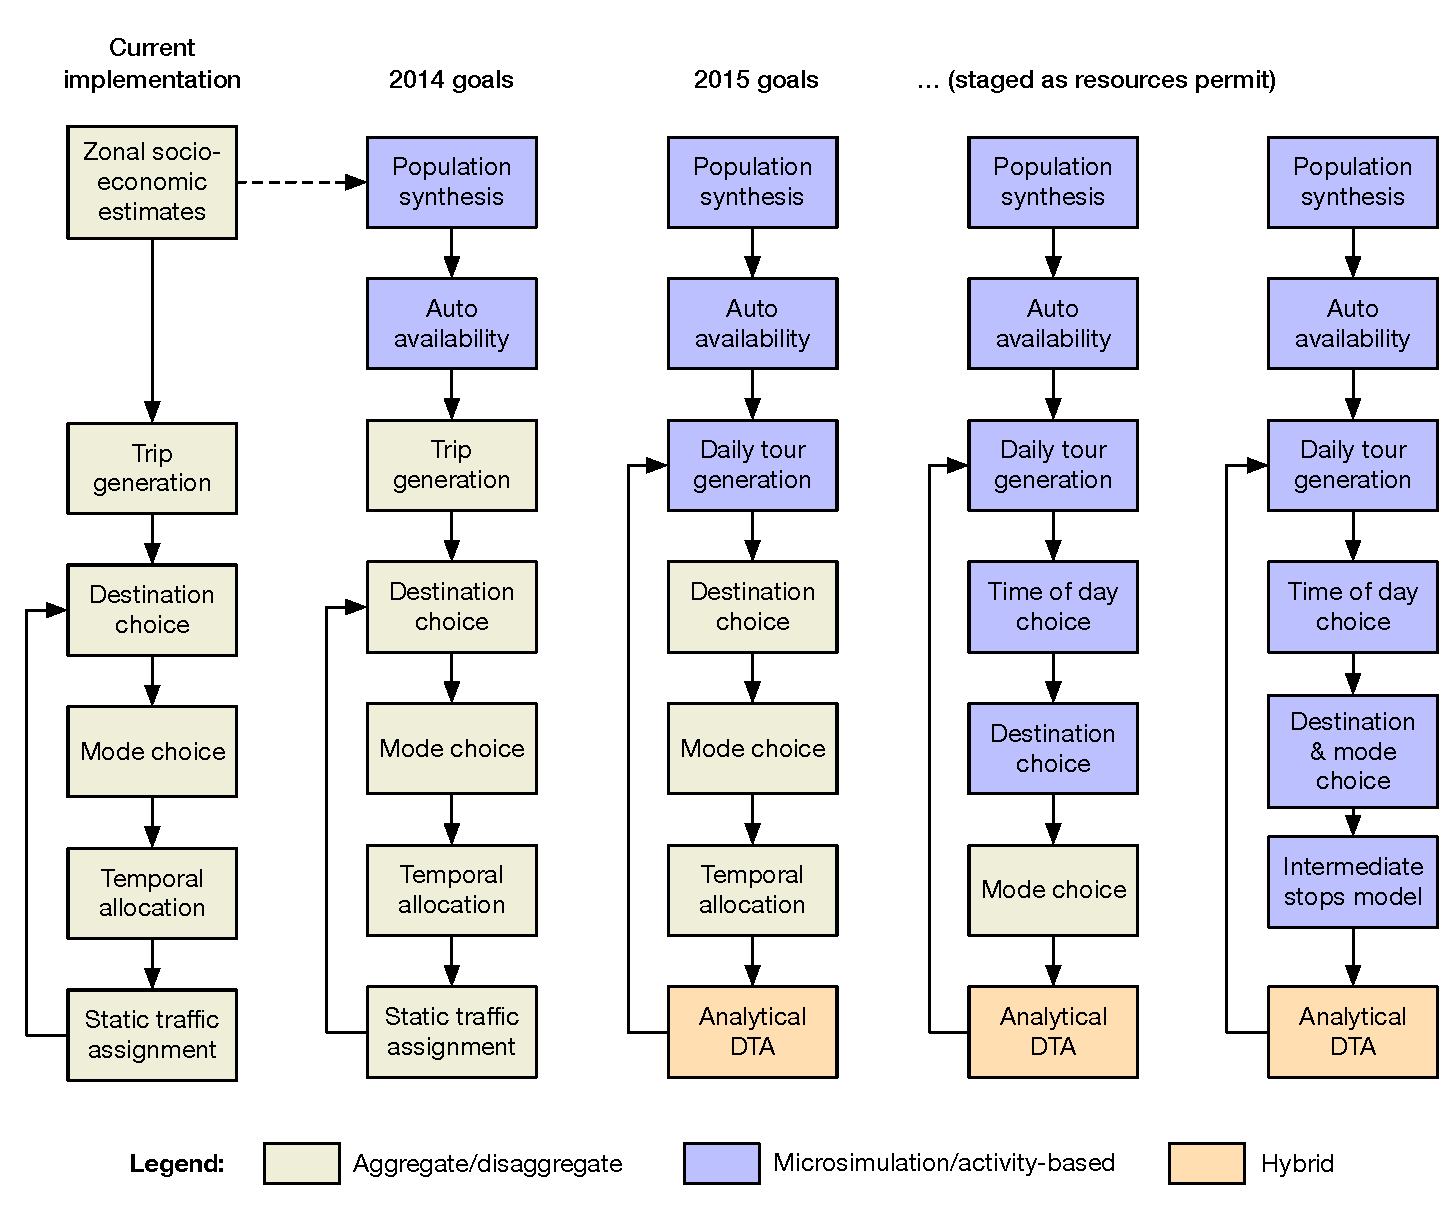
\includegraphics[width=6.5in]{graphics/44-maryland-model-evolution}
\caption{Transition from trip-based to activity-based framework in Maryland}
\label{fig:maryland-evolution}
\end{figure}

\subsection{Trip-based commercial vehicle models}

There is a considerable amount of literature devoted to freight modeling at several levels of resolution, ranging from urban truck models to inter-regional commodity flow models, to international trade forecasts. Most can be classified as either truck or commodity flow models, and local versus long-distance. The best practices in trip-based freight modeling are assembled in the FHWA \textit{Quick Response Freight Manual II} (QRFM)\citep{beagan07}, which use the same data required for person travel models. This approach can be coupled with the use of FAF to quickly implement trip-based statewide freight models. The techniques described can be quickly implemented, albeit only at coarse levels of FAF geography without additional processing of the data. How well such models work within statewide models has not been reported in the literature, although their shortcomings have been widely acknowledged. The trip generation and distribution parameter estimates from the manual can be updated with values from other areas, or iteratively adjusted to better match observed truck flows. Both can be undertaken at low cost.

Most states have few highly reliable vehicle classification counts, and typically none within urban areas other than on major highways. These are often supplemented with manual counts, counts from urban areas, and data from HPMS, most of which use adjustment factors derived from those few automatic traffic classifiers to impute the percentage of truck flows by area type and functional class. The experience of the authors is that few investments have as large a payoff as increasing the number of vehicle classification counts within the state. Most of these must be done by contractors, as resources to expand the number of automatic traffic recorders are not available. Data on the cost conducting such counts were not collected in this research, but the experience of the authors suggests the costs runs between \$150,000 to \$250,000 to expand the number of vehicle classification counts across a state to a level that permits robust model validation and insight into unique flow patterns.

Moving beyond the QRFM or comparable models and expanded count data requires a considerable investment in data. Establishment surveys that include truck travel diaries are often suggested to gain data that captures unique local patterns, obtain finer market segmentation, a wider range of explanatory variables, or capture of non-freight commercial vehicle travel. \cite{hunt07} used such data, collected at the cost of about \$3.5 million, to build a commercial vehicle model for Calgary. They have transferred their model to several other places, including the first-generation California statewide model. The cost seems surprisingly high, until one considers how different combinations of firm classifications, size ranges, and truck categories expand the number of observations required. The number of levels within each dimension can be reduced, of course, but only with corresponding increases in variances associated with parameters derived from the data.

Many argue that establishment surveys alone cannot provide a holistic view of all truck flows within a city or region, much less flows by all modes of transport. \cite{roorda11} proposes the fusion of shipper-based surveys with third-party truck tracking data to better understand truck patterns. \cite{zmud14} suggest investments in a combination of a revived Vehicle Inventory and Use Survey (VIUS), third-party truck tracking data, and agent-based modeling to achieve the same ends. California's investment in a replacement for the VIUS, described in \S\ref{sec:ca-statewide-models}, represents an essential first step in achieving those goals.

The cost of such data programs varies, and there is not enough experience with them to generalize the cost and effort involved in conducting them. However, it can confidently be asserted that they are multi-million dollar efforts whose design, testing, execution, and processing will likely last two to three years. They can be designed as continuous collection efforts rather than single large, costly, and disruptive activities. Moreover, the potential benefits of multi-state collaboration on such efforts seem enormous, but have not been attempted to date.

\subsection{Advanced commercial travel models}

The benefits of representing the tour structure of urban truck trips, and the associated improvements in functionality and outcomes, are well documented. There appears to be as much progress in implementing such models at the statewide level as there is within urban areas, in fact. Oregon developed a microsimulation-based short-distance truck tour model in 2003 that has been subsequently overhauled and adapted in Idaho and Ontario. A similar adaptation of the Calgary model was implemented in the Ohio statewide model a few years later \citep{gliebe07}. The Calgary model was also implemented in the California statewide model, as discussed in \S\ref{sec:ca-statewide-models}. The Calgary adaptations took advantage of extensive establishment survey data collected earlier in Alberta, and used in its original development. The adaptations were calibrated to match locally observed patterns.

The cost of implementing these four models ranged from \$75,000 to \$150,000, exclusive of the cost of obtaining and preparing the establishment survey. However, the cost is a bit misleading, for the integrated economic-land use-transport modeling platform they worked within provided additional data required to build and use them. Make and use coefficients derived from economic input-output data are used to associate commodities with industries, as well as estimates of production and consumption by firms with each sector. The Oregon model was implemented without the latter until recently, making it an open question of how much data are required to implement such models, versus desirable. If implemented outside of an integrated model it is likely that the data requirements would include the elements shown in Table \ref{tab:freight-data}.

\begin{table}[!t]   % 6
\centering
\caption{Typical data requirements for advanced freight models}
\label{tab:freight-data}
\begin{tabular}{L{1.9in}L{1.8in}L{2.3in}}
\hline
Data element & Scale & Estimated cost \\
\hline
Database of firms and key attributes (e.g., size, NAICS code, location) & Firms & \$5,000-\$30,000, depending upon vendor chosen and number of attributes desired \\
\gray Establishment travel survey & Firms segmented by area, industry, size, type of truck(s) operated or contracted & \$3.5M, but depends upon survey design, sampling frame and rate, and recruiting strategies \\
Forecast of gross state product, employment, and percentage of employees by occupation & State or sub-state region & Highly variable, depending on source, length and granularity of forecast periods, industry detail, etc. \\
\gray Make and use coefficients derived from input-output accounts & State or national & Typically included in economic forecast, but can be borrowed from other areas or derived from national benchmark IO accounts \\
Commercial vehicle survey (optional) & Trucks by operator & \$250,000 to \$2.5M, depending upon survey design, coverage, sampling rate, and other factors \\
\gray Vehicle tracking data (detailed GPS traces of truck movements over long periods) & Trucks by firm & Costs difficult to estimate because of only recent availability, cost in Florida and Ontario differ significantly \\
Carload Waybill Sample data (optional, used to better understand rail flows and calculate modal accessibilities) & Sampled waybills & Cost to obtain these data from Surface Transportation Board is minimal, although accompanied by non-disclosure requirements limiting their use \\
\hline
\end{tabular}
\end{table}

The costs shown reveal the substantial jump in cost and effort required to go from trip-based to advanced freight models. There is little ground in the middle, aside from substituting survey data collected elsewhere for locally collected information. Some states additionally represent rail flows, at least in aggregate, although analyses appear limited to the depiction of high-volume rail corridors and terminals. Thus, type and extent of data required will likely vary by type of model, modes of transport represented, resolution, and other factors. The data shown in Table \ref{tab:freight-data} should be used only as rough guidelines.

It is likely that more sophisticated freight models will eventually replace the current crop of models, both at the urban and statewide levels. \cite{chase13} outline the knowledge, data, models, and sharing required to improve the practice of freight modeling, although there are several competing proposals. A national freight model, if it were to come to fruition, would also dramatically change the freight modeling landscape, as well as substantially reducing the cost. Whether a given state can wait for those proposed initiatives to come to pass, or need to gain such capability earlier, is dictated by the issues and requirements they face.

\section{Urban-statewide model integration}\label{sec:urban-statewide-integration}

The approaches used for statewide modeling vary considerably, as noted in Chapter \ref{sec:survey-existing-practice}, especially with how they represent urban areas that have their own travel demand model. In some cases, statewide modelers attempt to use spatial, temporal, and behavioral resolutions more commonly found in urban areas, but stretched to cover the entire state. In other cases, a more abstract representation is used at the statewide level. Irrespective of the approach taken, it was expected that a great deal of effort would have gone into tightly integrating urban and statewide models. The use of common data would lend consistency to both models, even though each operated at different scales, and typically focused on different travel markets.

Instead, we found that such high-level coordination was rarely undertaken. Many states attempted to use aggregations of urban traffic analysis zones in areas where the two models overlapped, and many others reported a desire to replace external trip data and models at the urban level with long-distance travel data from the statewide model. However, many developers we interviewed expressed little need for or interest in tightly integrating urban and statewide models. It was felt that GIS techniques made conflation of demand data from heterogeneous zone systems practical when needed, yet freed developers of each model from having to coordinate the addition of new zones. The difficulties of maintaining a common network were cited even more frequently, suggesting that there was not as much overlap in the type and scale of analyses conducted with each modeling system as might be imagined. 

\section{Economic impact models}\label{sec:economic-impact-models}

Several states have adopted economic impact models to better inform project and program evaluations. Such platforms can be used to quantify the first and higher economic effects of proposed investments on the local and regional economy, multiplier effects, and potential revenue implications. Two examples of how statewide travel and economic impact models might interact are shown in Figure \ref{fig:economic-impact-models}. Indeed, some of the latter are as sophisticated as the former. The data requirements of these platforms will influence the design of the statewide model, as the value of seamless exchange of data is clear. There are no known instances of statewide models incorporating the results of these economic impact models, although the integrated models in Ohio and Oregon are designed to accept such feedback.

\begin{figure}[!t]   % 45
\centering
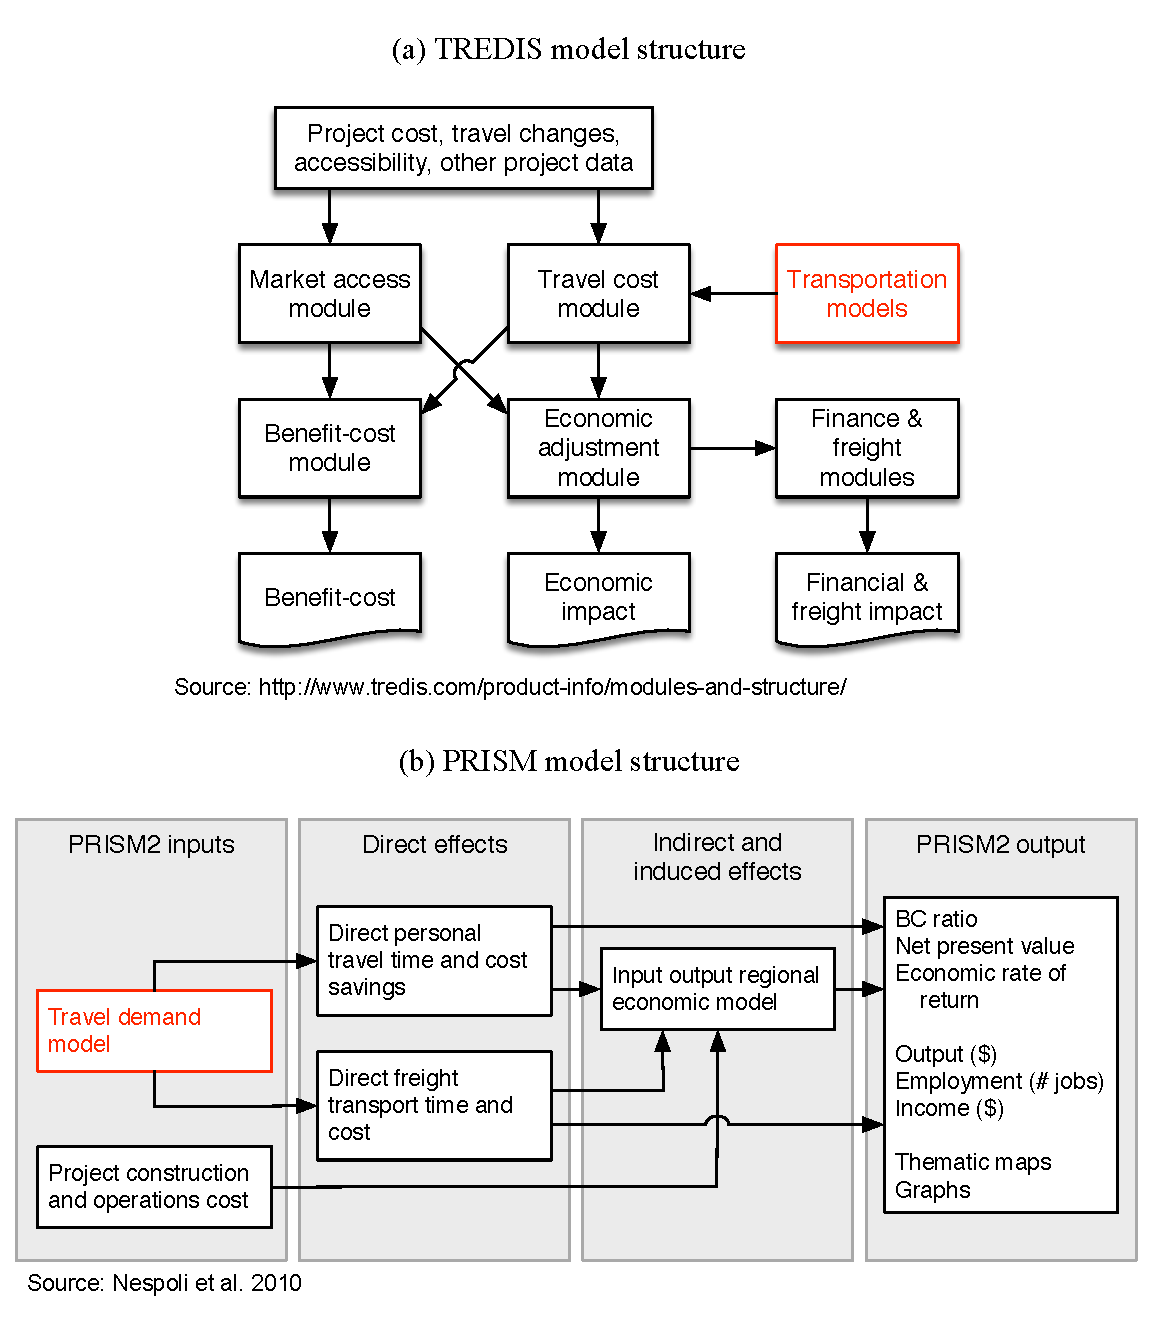
\includegraphics[scale=0.7]{graphics/45-economic-impact-models}
\caption{Examples of travel models within economic impact modeling frameworks}
\label{fig:economic-impact-models}
\end{figure}

The value of coupling statewide travel and economic impact models should not be dismissed. Oregon could use their statewide model to pose bridge deterioration as an economic issue affecting jobs, economic vitality, and market connectivity. It was not linked to an economic impact model, but because of its integrated economic-land use-transportation structure it could be used to demonstrate the impacts of bridge closures and restrictions. The Oregon legislature approved a \$4.8 billion bridge improvement program, based largely on the compelling evidence of economic impacts supplied by the statewide model. Couching an infrastructure problem as an economic issue was a wise move, for arguing the case based solely on the engineering issues was thought to have attracted far less support by legislators. It is a statewide modeling success story that deserves to be widely repeated, and a cogent reminder that a successful statewide modeling program should encompass more than just travel forecasting models.

\section{Model validation}

There is scant guidance on appropriate validation criteria for statewide models, or how they might be interpreted. Statewide modeling presents some unique challenges in this regard. The scant data available on long-distance travel and the unique characteristics of rural travelers dictates that they are consumed in model estimation and calibration, leaving few available for validation. This is even more true for commercial vehicles,  whose underlying business and travel patterns have much wider variances associated with them. The topic of freight model validation is rarely addressed in the literature, and definitive guidance on appropriate performance measures and testing procedures at either the urban or statewide level are lacking.

\cite{cambridge10} evaluated of validation practices and outcomes used in 11 of the 32 statewide models they reviewed, which remains a singular work in this area. They examined the structure and typical uses of these models, which revealed they covered wide ranges, precluding a single set of benchmark tests and standards. Differences in market segmentation frustrated attempts to isolate patterns in the data, and even otherwise similar models were found to have a wide range of reported parameter estimates. They cited several sources of data that could be used in validation, but the Highway Performance Monitoring System (HPMS) was the only one that is not commonly used in model development. We found no evidence in our review that validation practices have evolved since then.

The criteria used in different states were found to vary considerably, as shown in Figure \ref{fig:validation-practices}. Information from three additional models has been added by the authors, which does not change the earlier finding that most states relied solely upon measures of how well the modeled flows replicated observed flows. Statistical measures commonly used in urban models, such as root mean square error (RMSE) by functional class and count volume range and screenline comparisons, also dominated the evaluation of statewide models. Independent estimates of vehicle miles of travel by county from the HPMS are also widely used to test model performance. Comparisons of average auto occupancy were the only tests widely carried out beyond the assessment of traffic assignment outcomes.

\begin{figure}[!t]
\centering
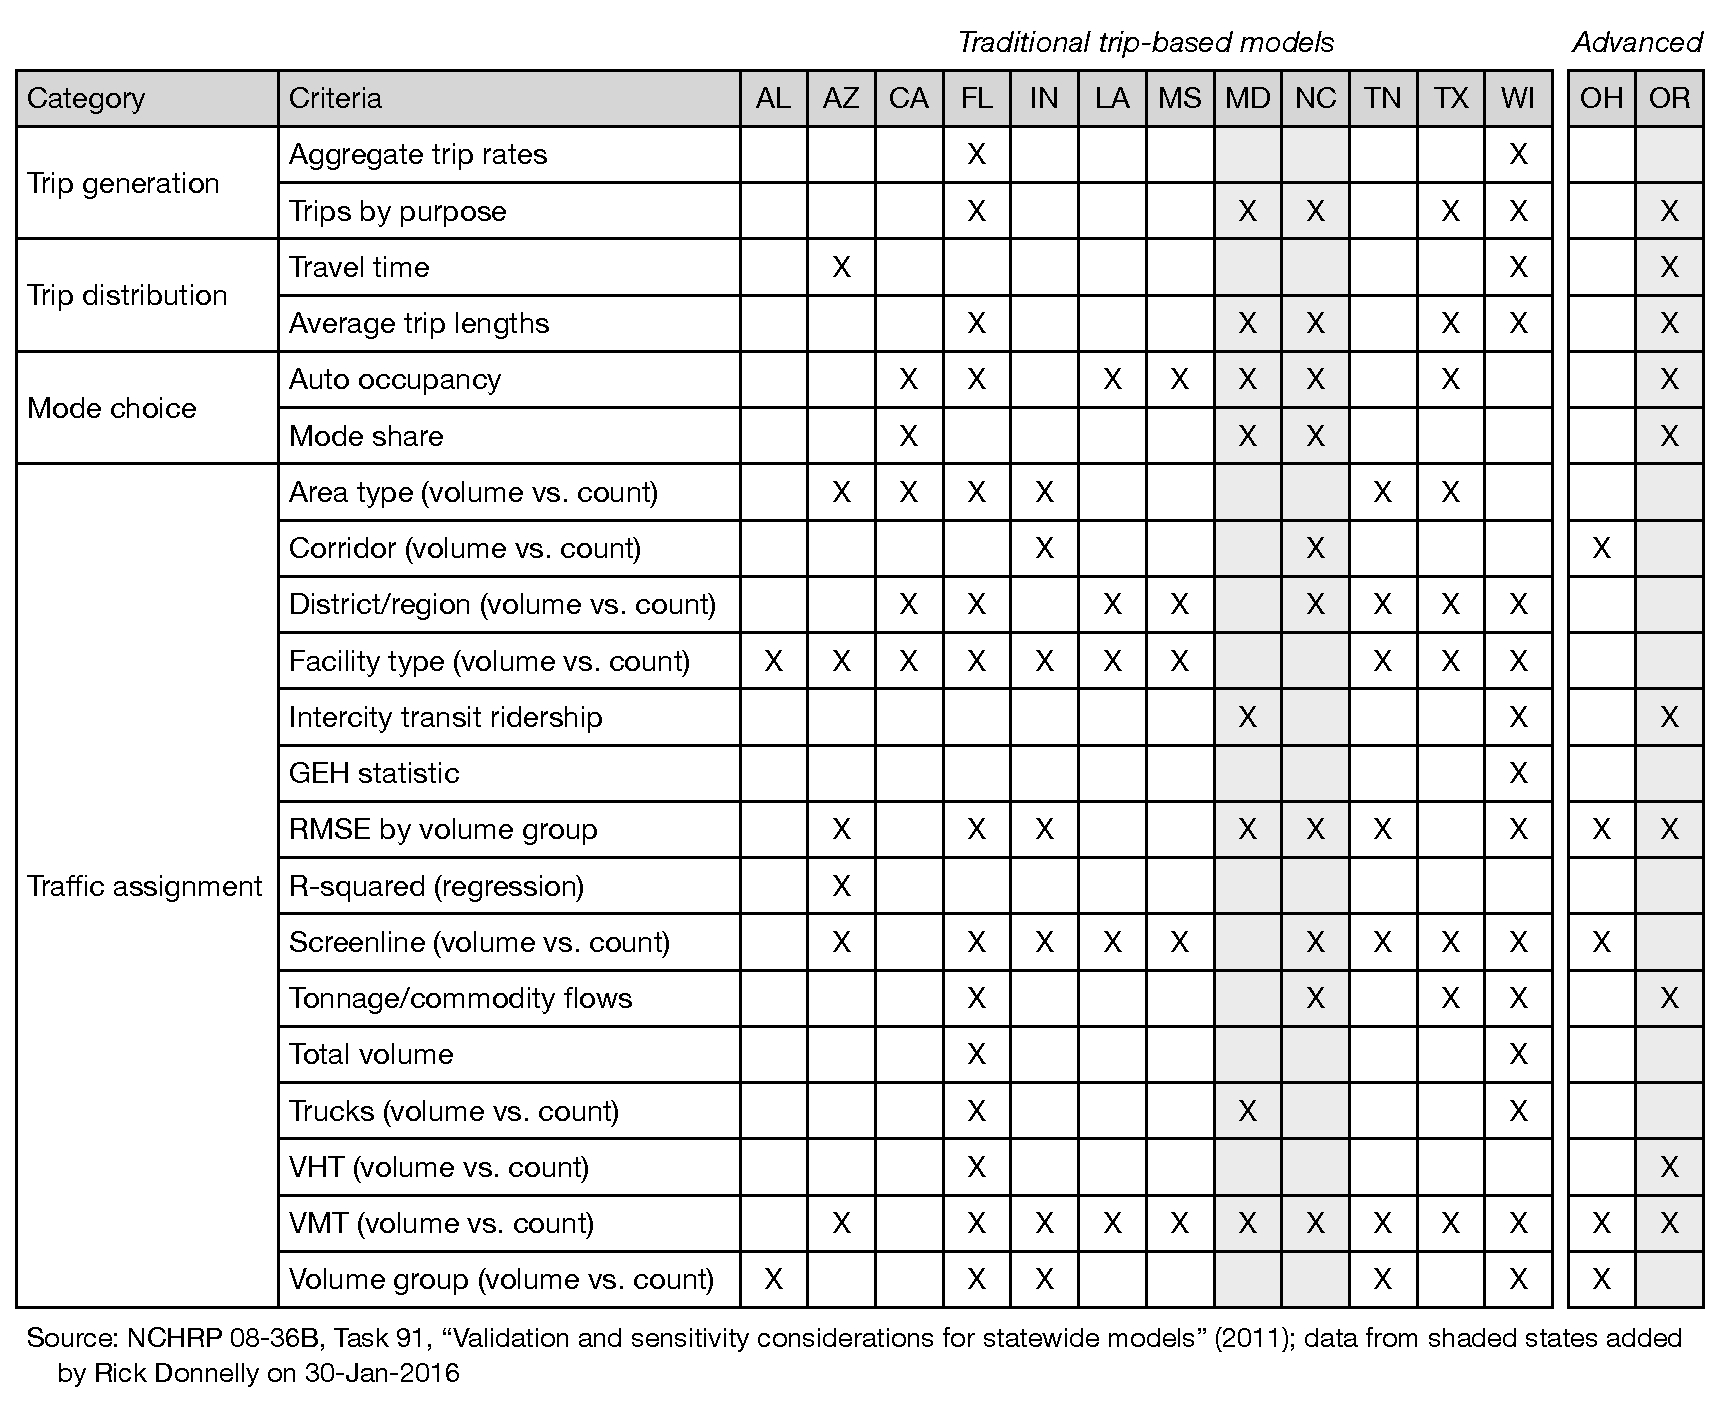
\includegraphics[width=6.5in]{graphics/46-validation-practices}
\caption{Validation practices employed in statewide modeling}
\label{fig:validation-practices}
\end{figure}

An examination of the validation outcomes revealed that statewide models tend to have larger assignment errors than typically encountered in urban models. This was attributed to the coarser networks typically used in statewide models and the correspondingly large traffic analysis zones, as well as low volumes outside urban areas. The latter typically have higher variances associated with them, which in turn limits how accurately they can be reproduced.

The authors of this report have converted the tabular comparison of percent RMSE within different count range reported, and added data from models they have more recent experience with, in Figure \ref{fig:prmse-comparisons}. This comparison is almost the only one that is consistently reported across all statewide models. The pattern is consistent and instructive, as well as the large influence of outliers for very low volume roads on the PRMSE scores. However, it remains only one of several that would be ideal for comparison across states. It is hoped that the excellent comparison conducted earlier is expanded in the future, for this is one area where statewide models remain behind accepted practice in urban modeling.

\begin{figure}
\centering
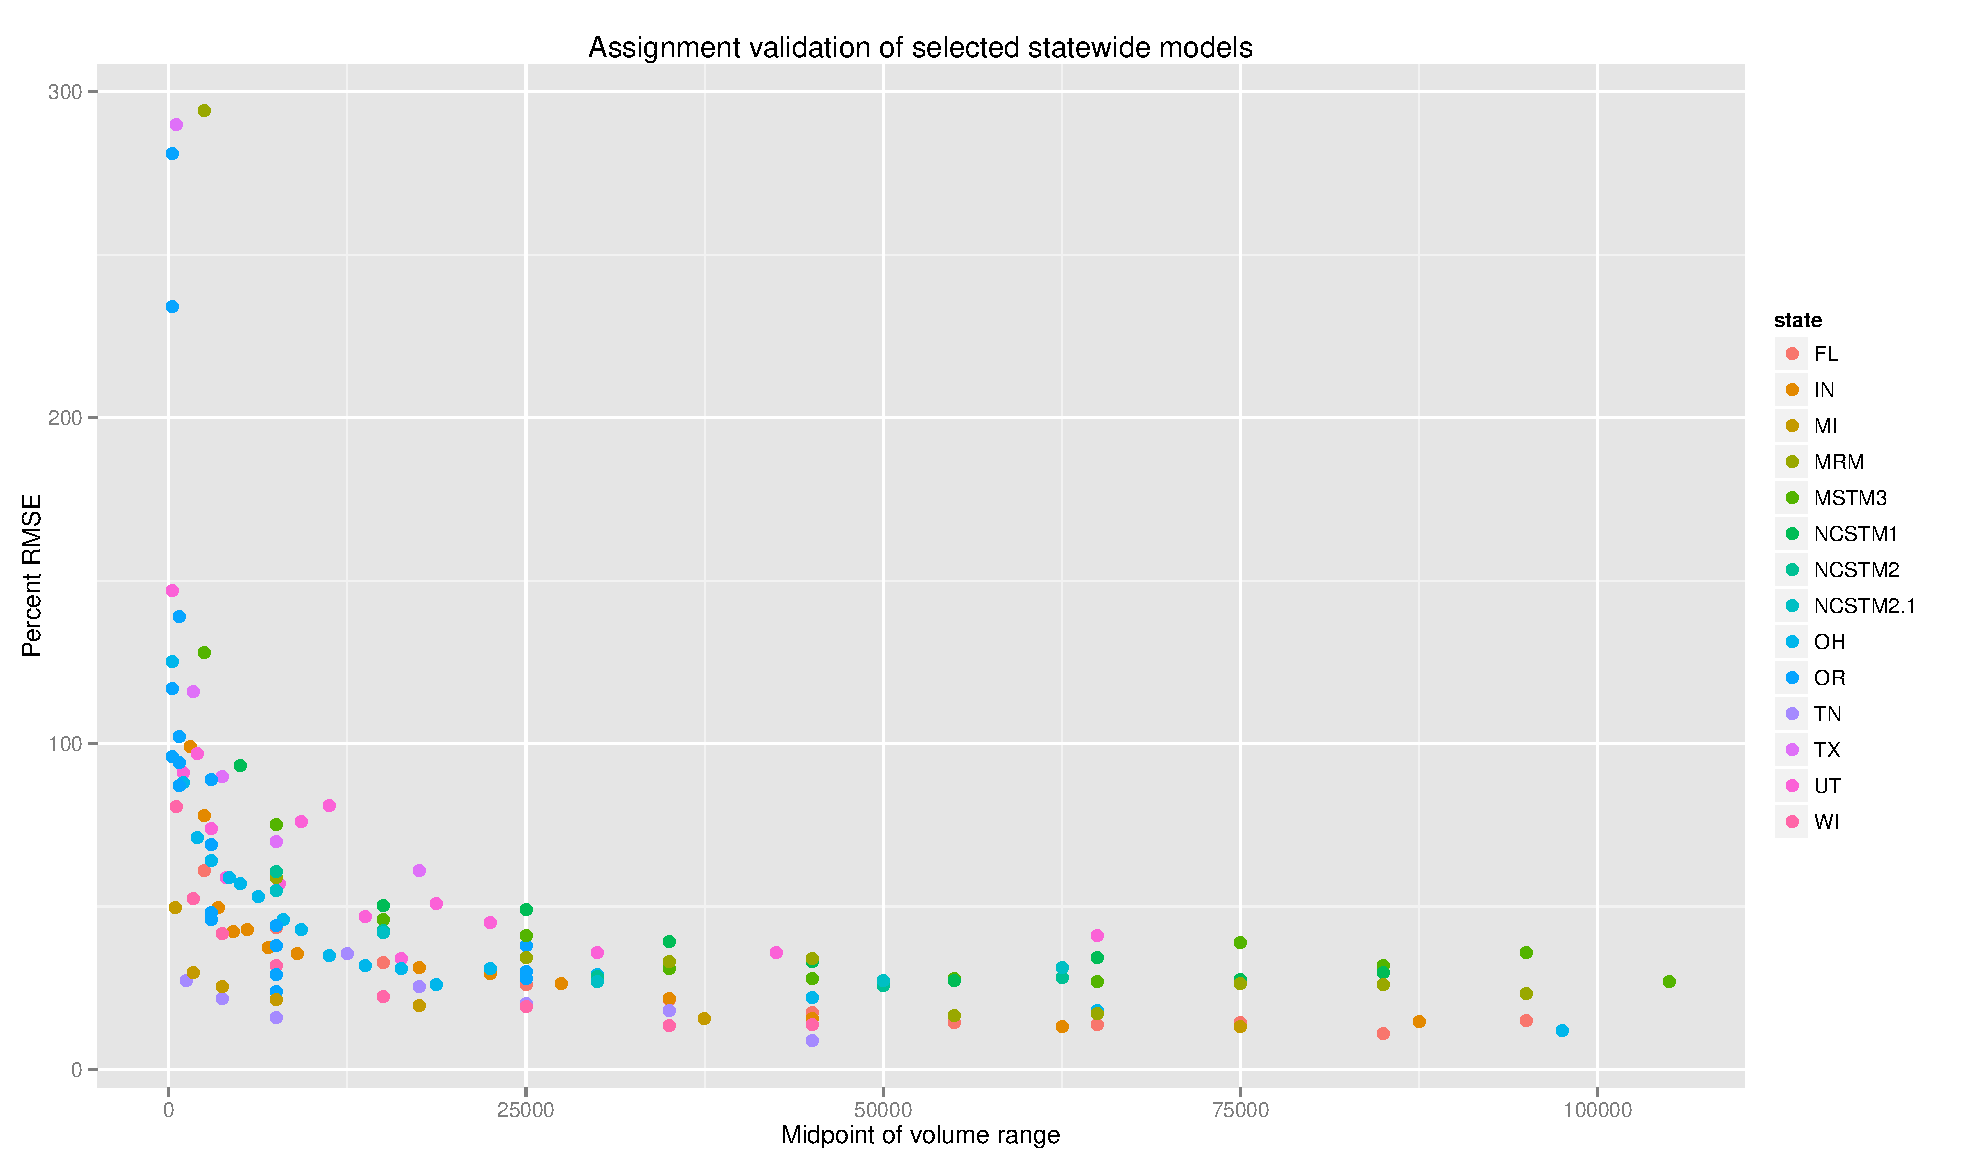
\includegraphics[width=6.5in]{graphics/47-prmse-comparisons}
\caption{Comparisons of percent RMSE by volume range for selected statewide models}
\label{fig:prmse-comparisons}
\end{figure}

\section{Computational burdens}

The 16-hour gold standard for statewide model runs --- the amount of time between when an analyst would start a run before leaving work and when they return to use its output the next morning --- is widely missed in many cases, especially those that cover large areas and populations, or have complex choice models. The urgency of addressing this issue was cited by several of the modelers encountered during the research for this report. This issue stems from a combination of factors:

\begin{itemize}
\item
The urge to build statewide models at the same levels of fidelity and resolution as urban models is strong. In some cases, this reflects the reductionist mindset of the model designer, but more often it is in response to needs to conduct fine-grained analyses of projects and corridors using statewide models. This need is particularly strong in areas of the state that are not covered by urban models, especially in corridors that connect two or more of them.
\item
The size of the state, both in land area and population, seems to correlate with the diversity and complexity of issues the models must be able to address. Thus, the already larger data and computational burdens imposed by the size of the networks and zone systems are compounded by more complex and complicated behavioral models.
\item
The overall trend in travel demand forecasting is towards a highly granular representation of agents and systems. Most advanced travel models work with synthetic households that are associated with much smaller zones than a decade ago, with the model operating on a continuous time scale or close to it. Some model the interaction between individual household members and their joint decisions. Such models are increasingly being coupled with dynamic traffic assignment models. Much of the evolving practice in urban travel modeling finds its way into statewide models, resulting in a slow creep of increasing detail in the latter.
\item
Advanced computational strategies remain out of reach for most model developers, whether they are using commercial software or not. No widely-accepted platform has emerged for the implementation of microsimulation-based advanced travel models, which are increasingly being used in statewide and urban modeling.
\end{itemize}

These realities leave statewide modelers with few choices for improving run-time performance, despite the frequent mention of the importance of improvements in this area. The lack of near-term options would seem to make this a modeling improvement priority.
